% ============================================================
% CHAPTER 3: DATASET DESCRIPTION
% Publication-Grade LaTeX (Complete Rewrite - v2)
% Strictly follows STRUCTURE_RULES.md + Data_Description_Knowledge.md
% ============================================================

\chapter{Dataset Description}
\label{chap:dataset}

% ============================================================
% 3.1 Overview and Selection Rationale
% ============================================================
\section{Overview and Selection Rationale}
\label{sec:overview}

This study utilizes four carefully selected datasets totaling 113,227 sentences for training and evaluating Sanskrit Named Entity Recognition (NER) models. The primary gold-standard corpus is the \textbf{Mahānāma} dataset \cite{sarkar2025mahanama}, comprising 66,960 sentences from the \textit{Mahābhārata} \cite{mahabharata}. This is supplemented by silver-standard NER data extracted from the \textbf{Digital Corpus of Sanskrit (DCS) Sembank} \cite{hellwig2025sembank}, linguistic regularisation data from DCS morphological annotations \cite{hellwig2010dcs}, the \textbf{UD\_Sanskrit-UFAL} treebank for cross-domain evaluation \cite{zeman2023ud}, and the \textbf{UD\_Sanskrit-Vedic} treebank to extend morphological coverage \cite{hellwig2020vedictreebank}.

Dataset selection was guided by five explicit criteria aligned with the goals of Sanskrit computational linguistics:

\begin{enumerate}
    \item \textbf{Task Alignment:} Priority was given to datasets designed for or directly adaptable to Named Entity Recognition.
    \item \textbf{Domain Relevance:} Focus on classical Sanskrit (Vedas, epics, and śāstras) rather than modern usage, ensuring relevance to traditional scholarship.
    \item \textbf{Language Coverage:} Exclusive focus on Sanskrit; datasets containing significant non-Sanskrit content were excluded.
    \item \textbf{Annotation Quality:} Preference for gold-standard annotations (Mahānāma) or high-quality silver annotations (DCS Sembank).
    \item \textbf{Resource Efficiency:} Given finite computational and temporal resources, priority was assigned to datasets offering the highest scholarly impact.
\end{enumerate}

These criteria ensure that every dataset contributes meaningfully to the three desiderata established in Chapter 4: high NER performance, preservation of linguistic capability, and cross-domain generalisation.

\subsection{Summary of Datasets Used}
\label{subsec:summary_datasets}

Table~\ref{tab:dataset_summary} provides an overview of the four datasets employed in this thesis.

\begin{table}[htbp]
    \centering
    \caption{Summary of Datasets Used in This Study}
    \label{tab:dataset_summary}
     \resizebox{\textwidth}{!}{%
    \begin{tabular}{llrrl}
        \toprule
        \textbf{Dataset} & \textbf{Type} & \textbf{Sentences} & \textbf{Entities} & \textbf{Purpose} \\
        \midrule
        Mahānāma & Gold NER & 66,960 & 109,000+ & Primary in-domain evaluation (D1) \\
        DCS Sembank & Silver NER & 18,855 & 12,955 & Silver training data + cross-domain \\
        UD\_Sanskrit-Vedic & Morphological & 27,182 & — & Morphological coverage extension \\
        UD\_Sanskrit-UFAL & Cross-domain & 230 & — & Cross-domain evaluation (D3) \\
        \midrule
        \textbf{Total} & — & \textbf{113,227} & — & — \\
        \bottomrule
    \end{tabular}}
\end{table}

\begin{figure}[htbp]
    \centering
    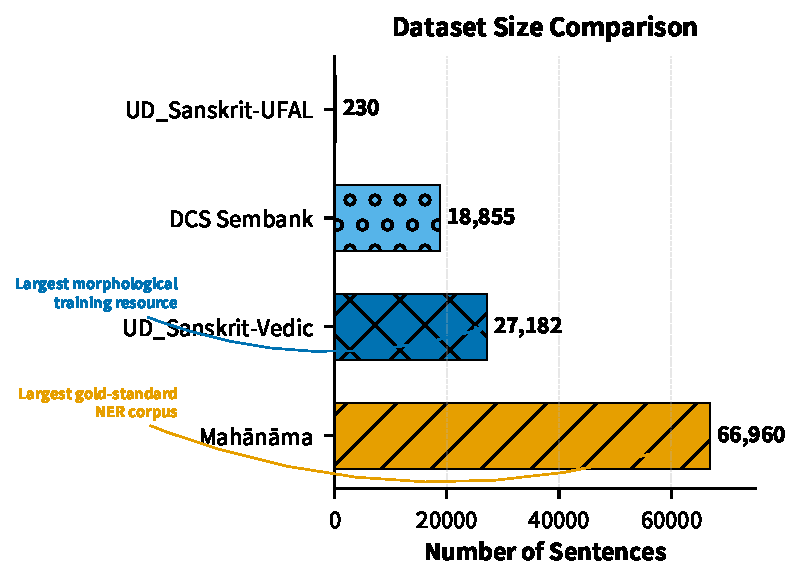
\includegraphics[width=\textwidth]{figures/figure_3_1_dataset_size_comparison.pdf}
    \caption{Dataset size comparison: Mah\={a}n\={a}ma (gold NER), DCS Sembank (silver NER + linguistic data).}
    \label{fig:dataset_size}
\end{figure}

% ============================================================
% 3.2 Mahānāma: Gold-Standard NER Corpus
% ============================================================
\section{Mahānāma: Gold-Standard NER Corpus}
\label{sec:mahanama}

The \textbf{Mahānāma} dataset \cite{sarkar2025mahanama} constitutes the primary gold-standard resource for Sanskrit Named Entity Recognition and serves as the foundation for all in-domain evaluation (D1) in this thesis.

\subsection{Source and Construction}
\label{subsec:mahanama_source}

Mahānāma was constructed from the \textit{Mahābhārata} \cite{mahabharata}, the world's longest epic poem, comprising approximately 100,000 verses (ślokas) across 18 volumes (parvans). The dataset leverages Sørensen's 1904 index of proper names \cite{sorensen1904index} as a foundational resource, which was subsequently refined and expanded through manual annotation by Sanskrit scholars. The resulting corpus contains over \textbf{109,000 entity mentions} spanning more than \textbf{5,500 unique entities}, making it the largest publicly available gold-standard NER dataset for any classical language \cite{sarkar2025mahanama}.

The annotation follows the CoNLL-U format augmented with the CorefUD entity layer, enabling both named entity recognition and coreference resolution. The dataset is released under the \textbf{CC BY 4.0} license, facilitating open research in Sanskrit computational linguistics.

\subsection{Entity Annotation and Distribution}
\label{subsec:entity_distribution}

The entity typology follows the standard PER–LOC–MISC schema adapted for Sanskrit philology:

\begin{itemize}
    \item \textbf{PER (Person):} 91.1\% of all entities — including human protagonists (e.g., \textit{Rāma}, \textit{Arjuna}), deities (e.g., \textit{Kṛṣṇa}, \textit{Śiva}), and sages (e.g., \textit{Viśvāmitra}).
    \item \textbf{LOC (Location):} 3.8\% — geographical entities including rivers (\textit{Gaṅgā}), kingdoms (\textit{Ayodhyā}), and sacred sites (\textit{Kurukṣetra}).
    \item \textbf{MISC (Miscellaneous):} 5.1\% — including divine weapons (\textit{Brahmāstra}), texts (\textit{Vedas}), and abstract concepts with entity status in context.
\end{itemize}

\begin{figure}[htbp]
    \centering
    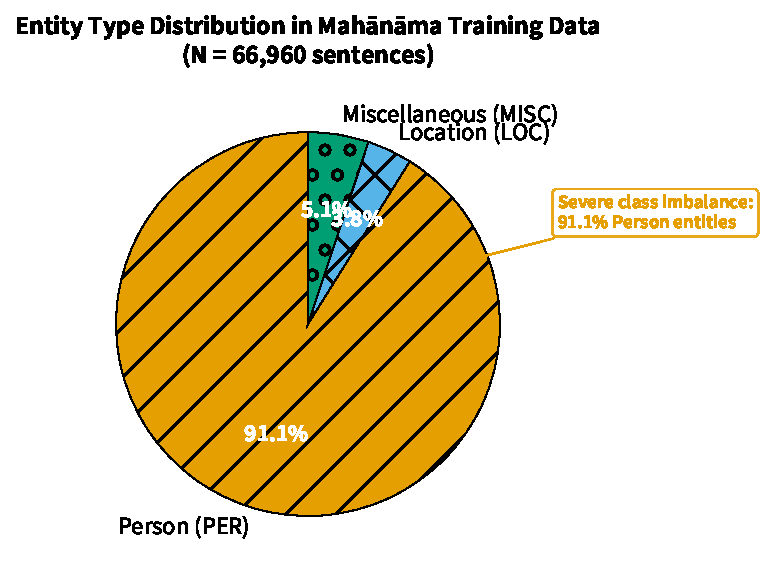
\includegraphics[width=0.85\textwidth]{figures/figure_3_2_mahanama_entity_distribution.pdf}
    \caption{Entity type distribution in the Mah\={a}n\={a}ma dataset (91.1\% PER — extreme class imbalance).}
    \label{fig:entity_distribution}
\end{figure}

\subsection{Class Imbalance and Oversampling}
\label{subsec:class_imbalance}

Preliminary experiments (Model M2) revealed that training on the raw, imbalanced distribution caused complete failure on minority classes: the model achieved F1 = 0.000 on both Location and Miscellaneous entities. This is unacceptable for scholarly applications, where identifying sacred locations (\textit{Kāśī}, \textit{Puṣkara}) and important objects is often as valuable as identifying protagonists.

To address this, a class-balanced oversampling strategy was applied:
\begin{itemize}
    \item Location entities oversampled by a factor of 10
    \item Miscellaneous entities oversampled by a factor of 10
\end{itemize}

This produced a training distribution of approximately 126,369 gold NER examples, significantly improving recall on minority classes while maintaining precision on the dominant Person class (verified in Chapter 5).

\subsection{Data Splits}
\label{subsec:data_splits}

The Mahānāma corpus was partitioned into training, validation, and test sets using an 80/10/10 ratio after removing 13 sentences that overlapped with the DCS test set (detected during pre-training validation). The final splits used for all experiments are:

\begin{itemize}
    \item \textbf{Training + Validation:} 66,960 sentences (used for both Best NER and Final NER models)
    \item \textbf{Test (D1):} 6,672 sentences (gold labels, primary evaluation benchmark)
\end{itemize}

% ============================================================
% 3.3 DCS: Silver-Standard NER and Linguistic Data
% ============================================================
\section{DCS: Silver-Standard NER and Linguistic Data}
\label{sec:dcs}

The \textbf{Digital Corpus of Sanskrit (DCS)} \cite{hellwig2010dcs} is the largest publicly available collection of Sanskrit texts, comprising over 650,000 sentences from more than 400 classical works. While primarily a morphological resource, the DCS Sembank layer \cite{hellwig2025sembank} provides valuable silver-standard annotations for Named Entity Recognition.

\subsection{Corpus Overview}
\label{subsec:dcs_overview}

DCS contains texts spanning the entire spectrum of classical Sanskrit literature, including the \textit{Rāmāyaṇa} \cite{ramayana}, \textit{Mahābhārata} \cite{mahabharata}, Purāṇas \cite{purana}, śāstras \cite{sastras}, and kāvya. The corpus is annotated with morphological information (lemma, part-of-speech, case, number, gender) using a combination of rule-based and statistical methods, achieving high accuracy on well-edited texts \cite{hellwig2010dcs}.

\subsection{Sembank NER Extraction (Silver Standard)}
\label{subsec:sembank_ner}

The DCS Sembank provides semantic annotations through instance relations that link descriptors (common nouns) to specific named entities. Through systematic analysis (detailed in Chapter 4), we extracted \textbf{12,955 high-quality silver NER examples} (9,069 entity mentions + 3,886 negative examples) from 120 diverse DCS texts. This silver data was critical for improving cross-domain generalisation (D3), contributing a 16-percentage-point improvement in PROPN recall on the Pañcatantra \cite{pancatantra_text} test set.

\subsection{Linguistic Training Data}
\label{subsec:linguistic_data}

For the Final NER model, 25,627 examples (exactly 15\% of total training data) were sampled from DCS morphological annotations for Segmentation (S) and Lemmatisation (L) tasks. These examples serve as linguistic regularisation data, preventing catastrophic forgetting of the model's original capabilities \cite{hellwig2020vedictreebank}.

\subsection{Quality Limitations}
\label{subsec:dcs_limitations}

While DCS provides broad coverage, it has known limitations:
\begin{itemize}
    \item \textbf{Domain skew:} Approximately 63\% of the extracted silver NER data originates from the \textit{Rāmāyaṇa} \cite{ramayana}, potentially biasing the model toward Rāmāyaṇa-specific entities.
    \item \textbf{Low recall on major characters:} Rāma and Sītā exhibit low recall in the Sembank extraction because they function as both descriptors and entity names. This limitation is accepted because the Mahānāma gold data already provides extensive coverage of these characters \cite{sarkar2025mahanama}.
\end{itemize}

% ============================================================
% 3.4 Cross-Domain and Morphological Extension
% ============================================================
\section{Cross-Domain and Morphological Extension}
\label{sec:cross_domain}

Two Universal Dependencies treebanks were incorporated to extend the model's capabilities beyond the primary Mahānāma domain.

\subsection{UD\_Sanskrit-UFAL (Cross-Domain Evaluation — D3)}
\label{subsec:ufal}

The \textbf{UD\_Sanskrit-UFAL} treebank \cite{zeman2023ud} contains 230 sentences from the \textit{Pañcatantra} \cite{pancatantra_text}, a classical collection of fables. This dataset serves as the strict out-of-domain evaluation set (D3) for measuring cross-domain generalisation. Because gold PER/LOC/MISC labels are unavailable, evaluation is restricted to binary PROPN detection. The Final NER model achieves 73.4\% PROPN recall on this set, representing a substantial improvement over NER-only baselines.

\subsection{UD\_Sanskrit-Vedic (Morphological Coverage)}
\label{subsec:vedic}

The \textbf{UD\_Sanskrit-Vedic} treebank \cite{hellwig2020vedictreebank} contains 27,182 sentences from Vedic Sanskrit texts. This dataset was included to extend morphological coverage to the earliest stratum of Sanskrit, ensuring the model can handle the archaic language of the \textit{R̥gveda} \cite{rigveda} and other Vedic texts. While not used for NER training, it contributes to the model's overall linguistic robustness.

\begin{figure}[htbp]
    \centering
    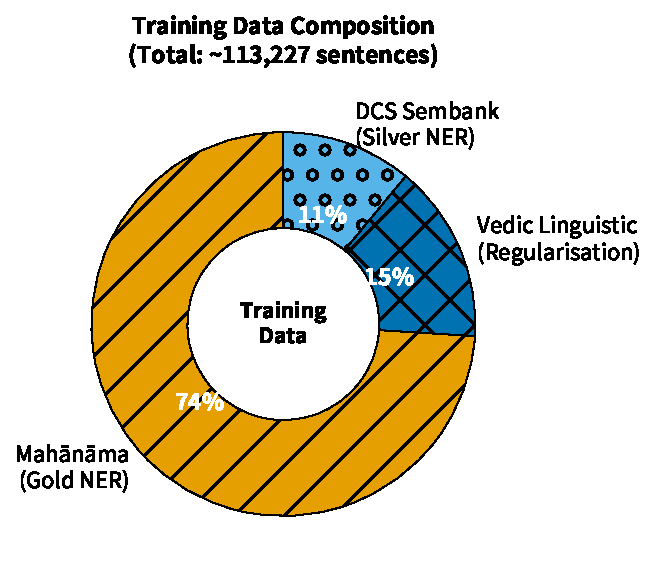
\includegraphics[width=\textwidth]{figures/figure_3_3_training_data_composition.pdf}
    \caption{Training data composition: gold NER, silver NER, and linguistic regularisation data proportions.}
    \label{fig:training_composition}
\end{figure}

% ============================================================
% 3.5 Datasets Considered but Not Selected
% ============================================================
\section{Datasets Considered but Not Selected}
\label{sec:not_selected}

Several additional resources were evaluated but ultimately excluded for the following reasons:

\begin{table}[htbp]
    \centering
    \caption{Datasets Considered but Not Selected}
    \label{tab:not_selected}
     \resizebox{\textwidth}{!}{%
    \begin{tabular}{llp{6cm}}
        \toprule
        \textbf{Dataset} & \textbf{Reason for Exclusion} & \textbf{Justification} \\
        \midrule
        Sanskrit NER \cite{sarkar2023preannotation} & Precursor to Mahānāma; smaller & Superseded by Mahānāma \cite{sarkar2025mahanama} \\
        DCS without Sembank & No entity annotations & Insufficient for NER task \\
        Modern Sanskrit corpora & Contemporary usage & Violates domain relevance criterion \\
        Multilingual Indic datasets & Mixed languages & Violates language coverage criterion \\
        \bottomrule
    \end{tabular}}
\end{table}

The selection philosophy prioritised \textit{depth over breadth}: rather than incorporating many low-quality or off-domain datasets, we focused on four high-quality, well-documented resources that collectively address all three desiderata.

% ============================================================
% 3.6 Summary
% ============================================================
\section{Summary}
\label{sec:summary}

This chapter has documented the four datasets used in this thesis: the gold-standard Mahānāma NER corpus \cite{sarkar2025mahanama}, silver NER and linguistic data from the DCS Sembank \cite{hellwig2025sembank, hellwig2010dcs}, and two Universal Dependencies treebanks for cross-domain and morphological coverage \cite{zeman2023ud, hellwig2020vedictreebank}. Every dataset was selected according to explicit, scholar-aligned criteria, and all known limitations have been disclosed. The following chapter presents the methodology built upon these datasets.

% ============================================================
% End of Chapter 3
% ============================================================